% ------------------------------------------------------------------------------
% TYPO3 CMS 8.6 - What's New - Chapter "Backend User Interface" (Spanish Version)
%
% @author	Michael Schams <schams.net>
% @license	Creative Commons BY-NC-SA 3.0
% @link		http://typo3.org/download/release-notes/whats-new/
% @language	English
% ------------------------------------------------------------------------------
% LTXE-CHAPTER-UID:		07b25346-95b1df21-a6ebe09a-49f53f41
% LTXE-CHAPTER-NAME:	Backend User Interface
% ------------------------------------------------------------------------------

\section{Backend User Interface}
\begin{frame}[fragile]
	\frametitle{Interfaz de Usuario de Backend}

	\begin{center}\huge{Capítulo 1:}\end{center}
	\begin{center}\huge{\color{typo3darkgrey}\textbf{Interfaz de Usuario de Backend}}\end{center}

\end{frame}

% ------------------------------------------------------------------------------
% LTXE-SLIDE-START
% LTXE-SLIDE-UID:		588f349d-075af1df-fedcd228-92f49b4a
% LTXE-SLIDE-ORIGIN:	4141a9cc-46da51df-9dd87a8b-9b15ac29 English
% LTXE-SLIDE-TITLE:		#12211: Scheduler Page Browser
% LTXE-SLIDE-REFERENCE:	!Feature: #12211 - Usability: Scheduler provide page browser to choose start page
% ------------------------------------------------------------------------------
\begin{frame}[fragile]
	\frametitle{Interfaz de Usuario de Backend}
	\framesubtitle{Navegador de Página del Programador}

	Para mejorar la usabilidad de la tarea de programador de \textbf{EXT:linkvalidator},
	el navegador de página fue añadido para seleccionar la página de inicio.

	\begin{figure}\vspace{-0.2cm}
		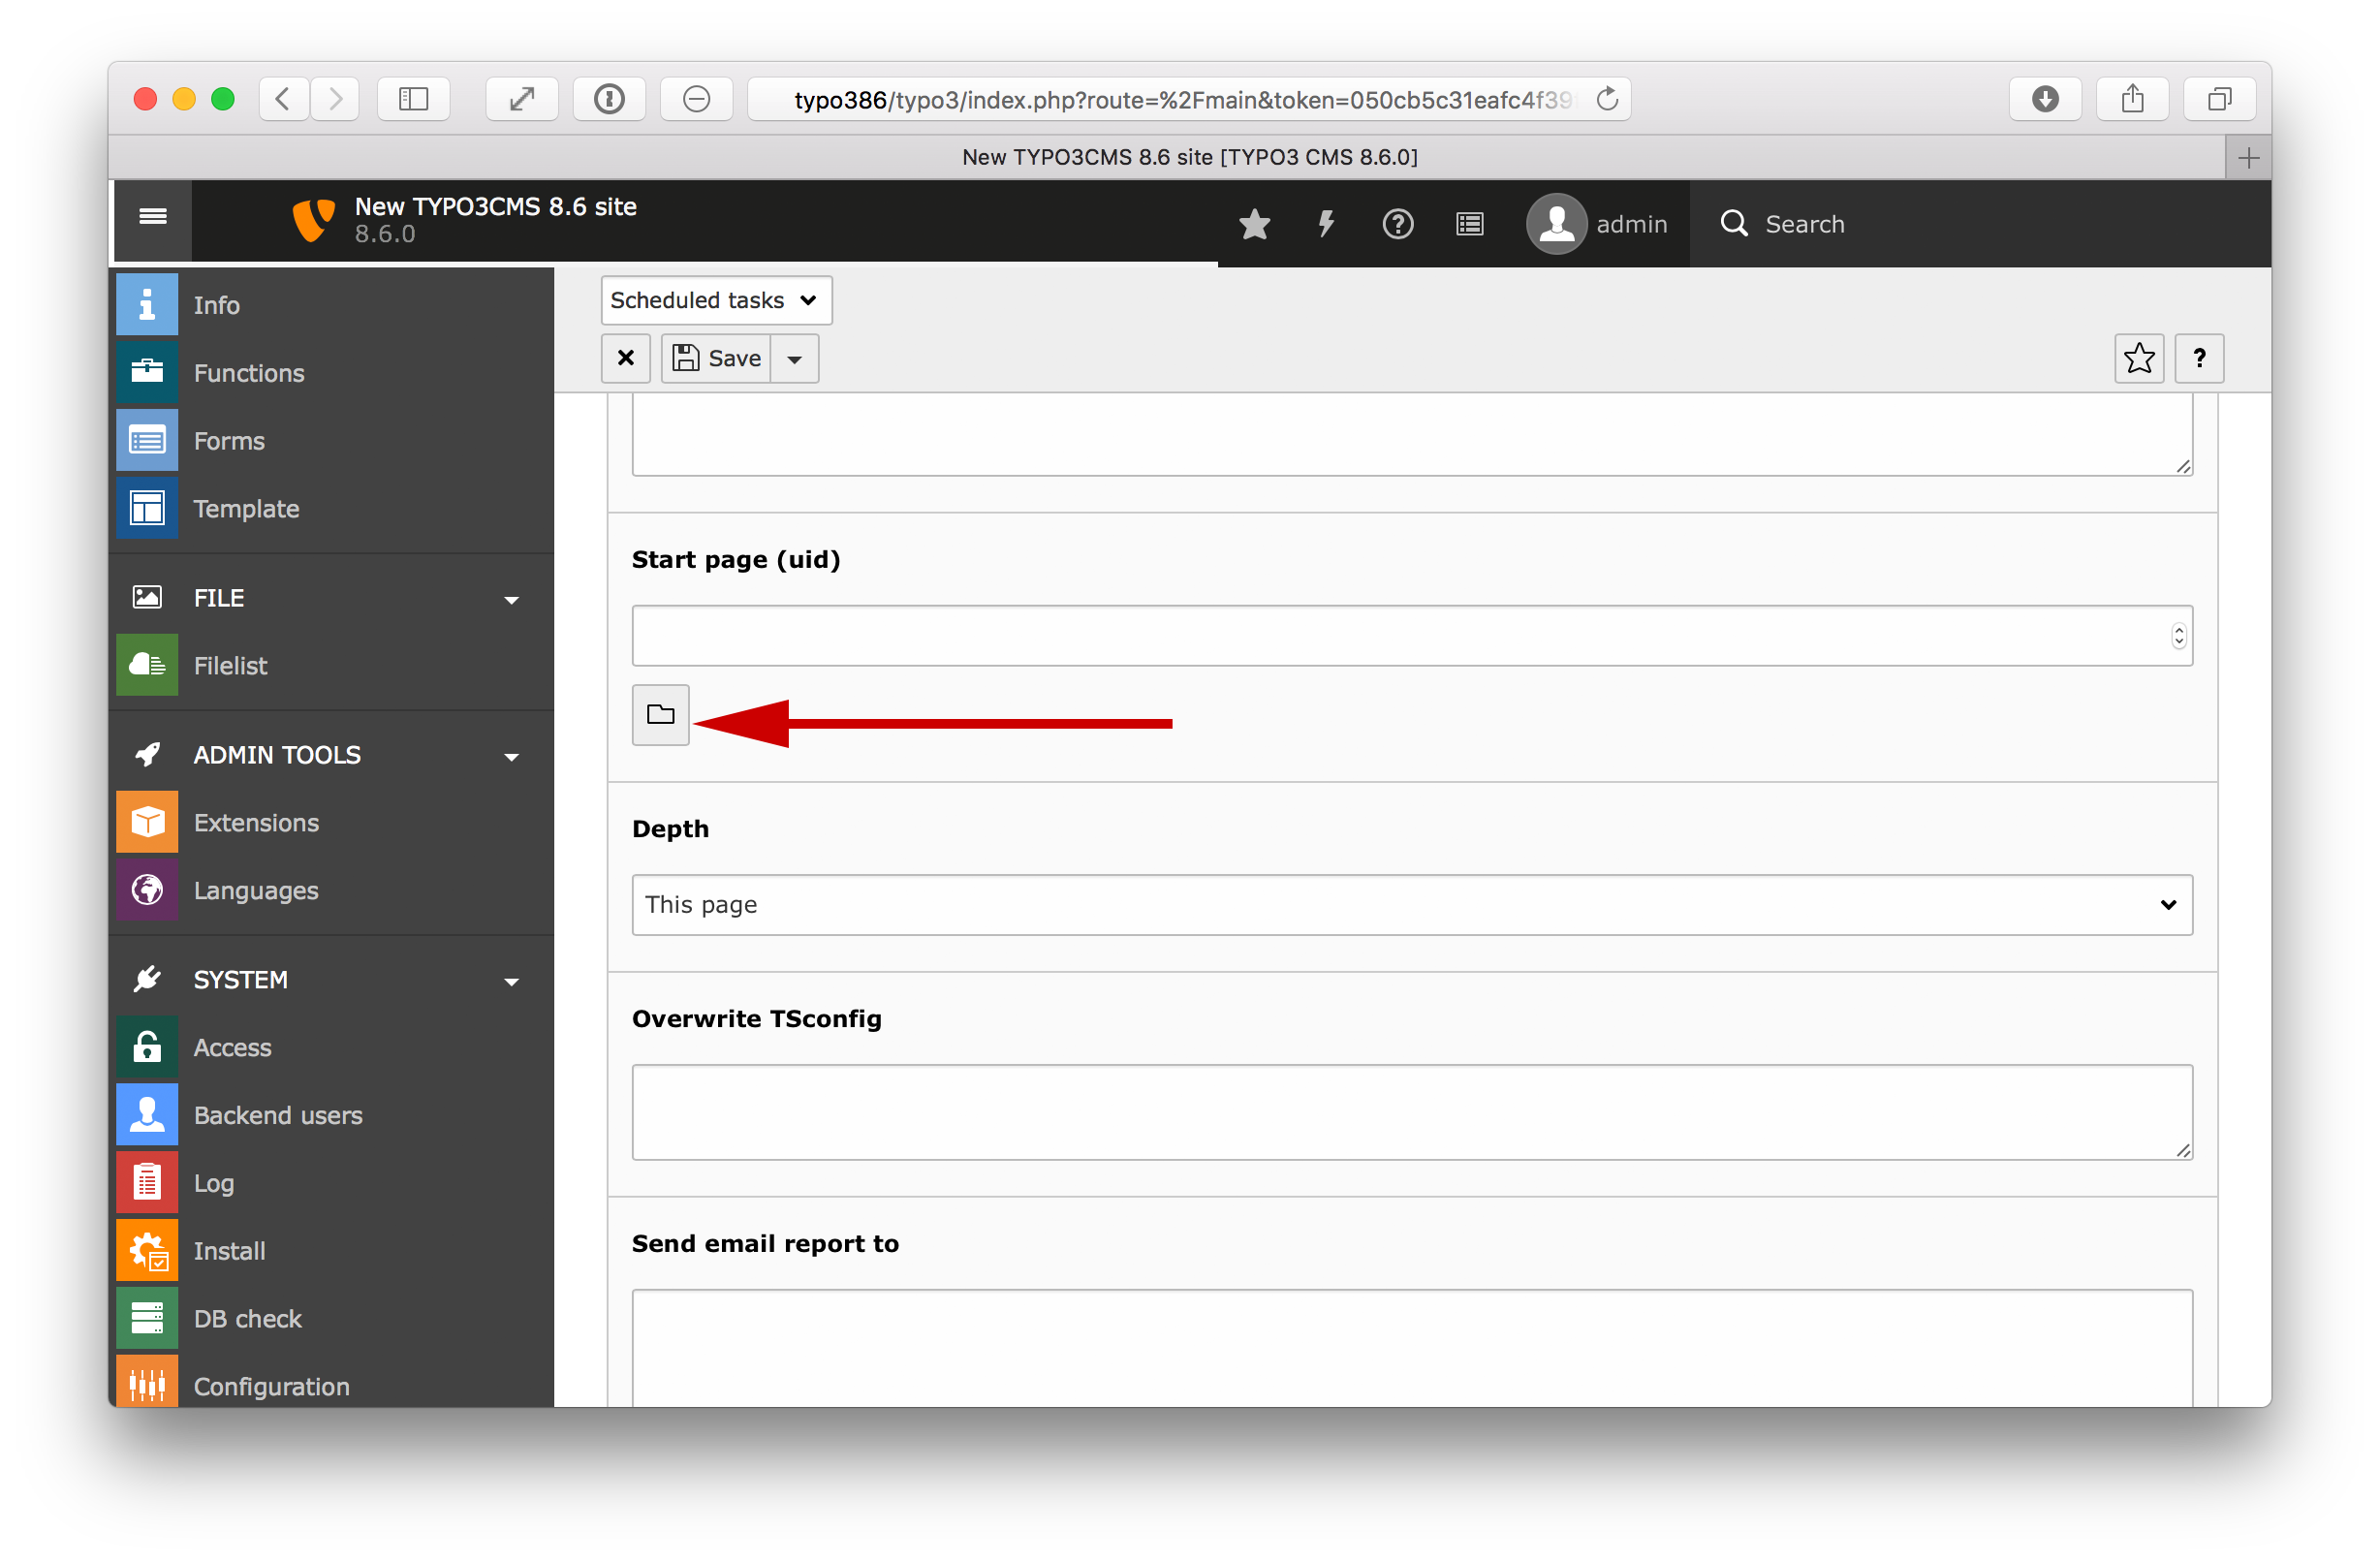
\includegraphics[width=0.67\linewidth]{BackendUserInterface/12211.png}
	\end{figure}

\end{frame}

% ------------------------------------------------------------------------------
% LTXE-SLIDE-START
% LTXE-SLIDE-UID:		644d6546-6e0691d9-8db22254-849d3fd6
% LTXE-SLIDE-ORIGIN:	f924be39-75ae40d9-ba00f0a8-3a6de040 English
% LTXE-SLIDE-TITLE:		#45537: Manually executed tasks
% LTXE-SLIDE-REFERENCE:	!Feature: #45537 - Run manually executed tasks on next cron-run
% ------------------------------------------------------------------------------
\begin{frame}[fragile]
	\frametitle{Interfaz de Usuario de Backend}
	\framesubtitle{Lanzar Tareas Ejecutadas Manualmente el Siguiente Lanzamiento del Cron}

	\begin{columns}[T]
		\begin{column}{0.3\textwidth}
			Hay un nuevo icono de acción para marcar una tarea para que se ejecute por cron. También un nuevo botón
			"Ejecutar tareas seleccionadas en el siguiente trabajo del cron" ha sido añadido para marcar todas las acciones selecionadas
			y que corran en el siguiente trabajo del cron.
		\end{column}

		\begin{column}{0.7\textwidth}
			\begin{figure}\vspace{-0.6cm}
				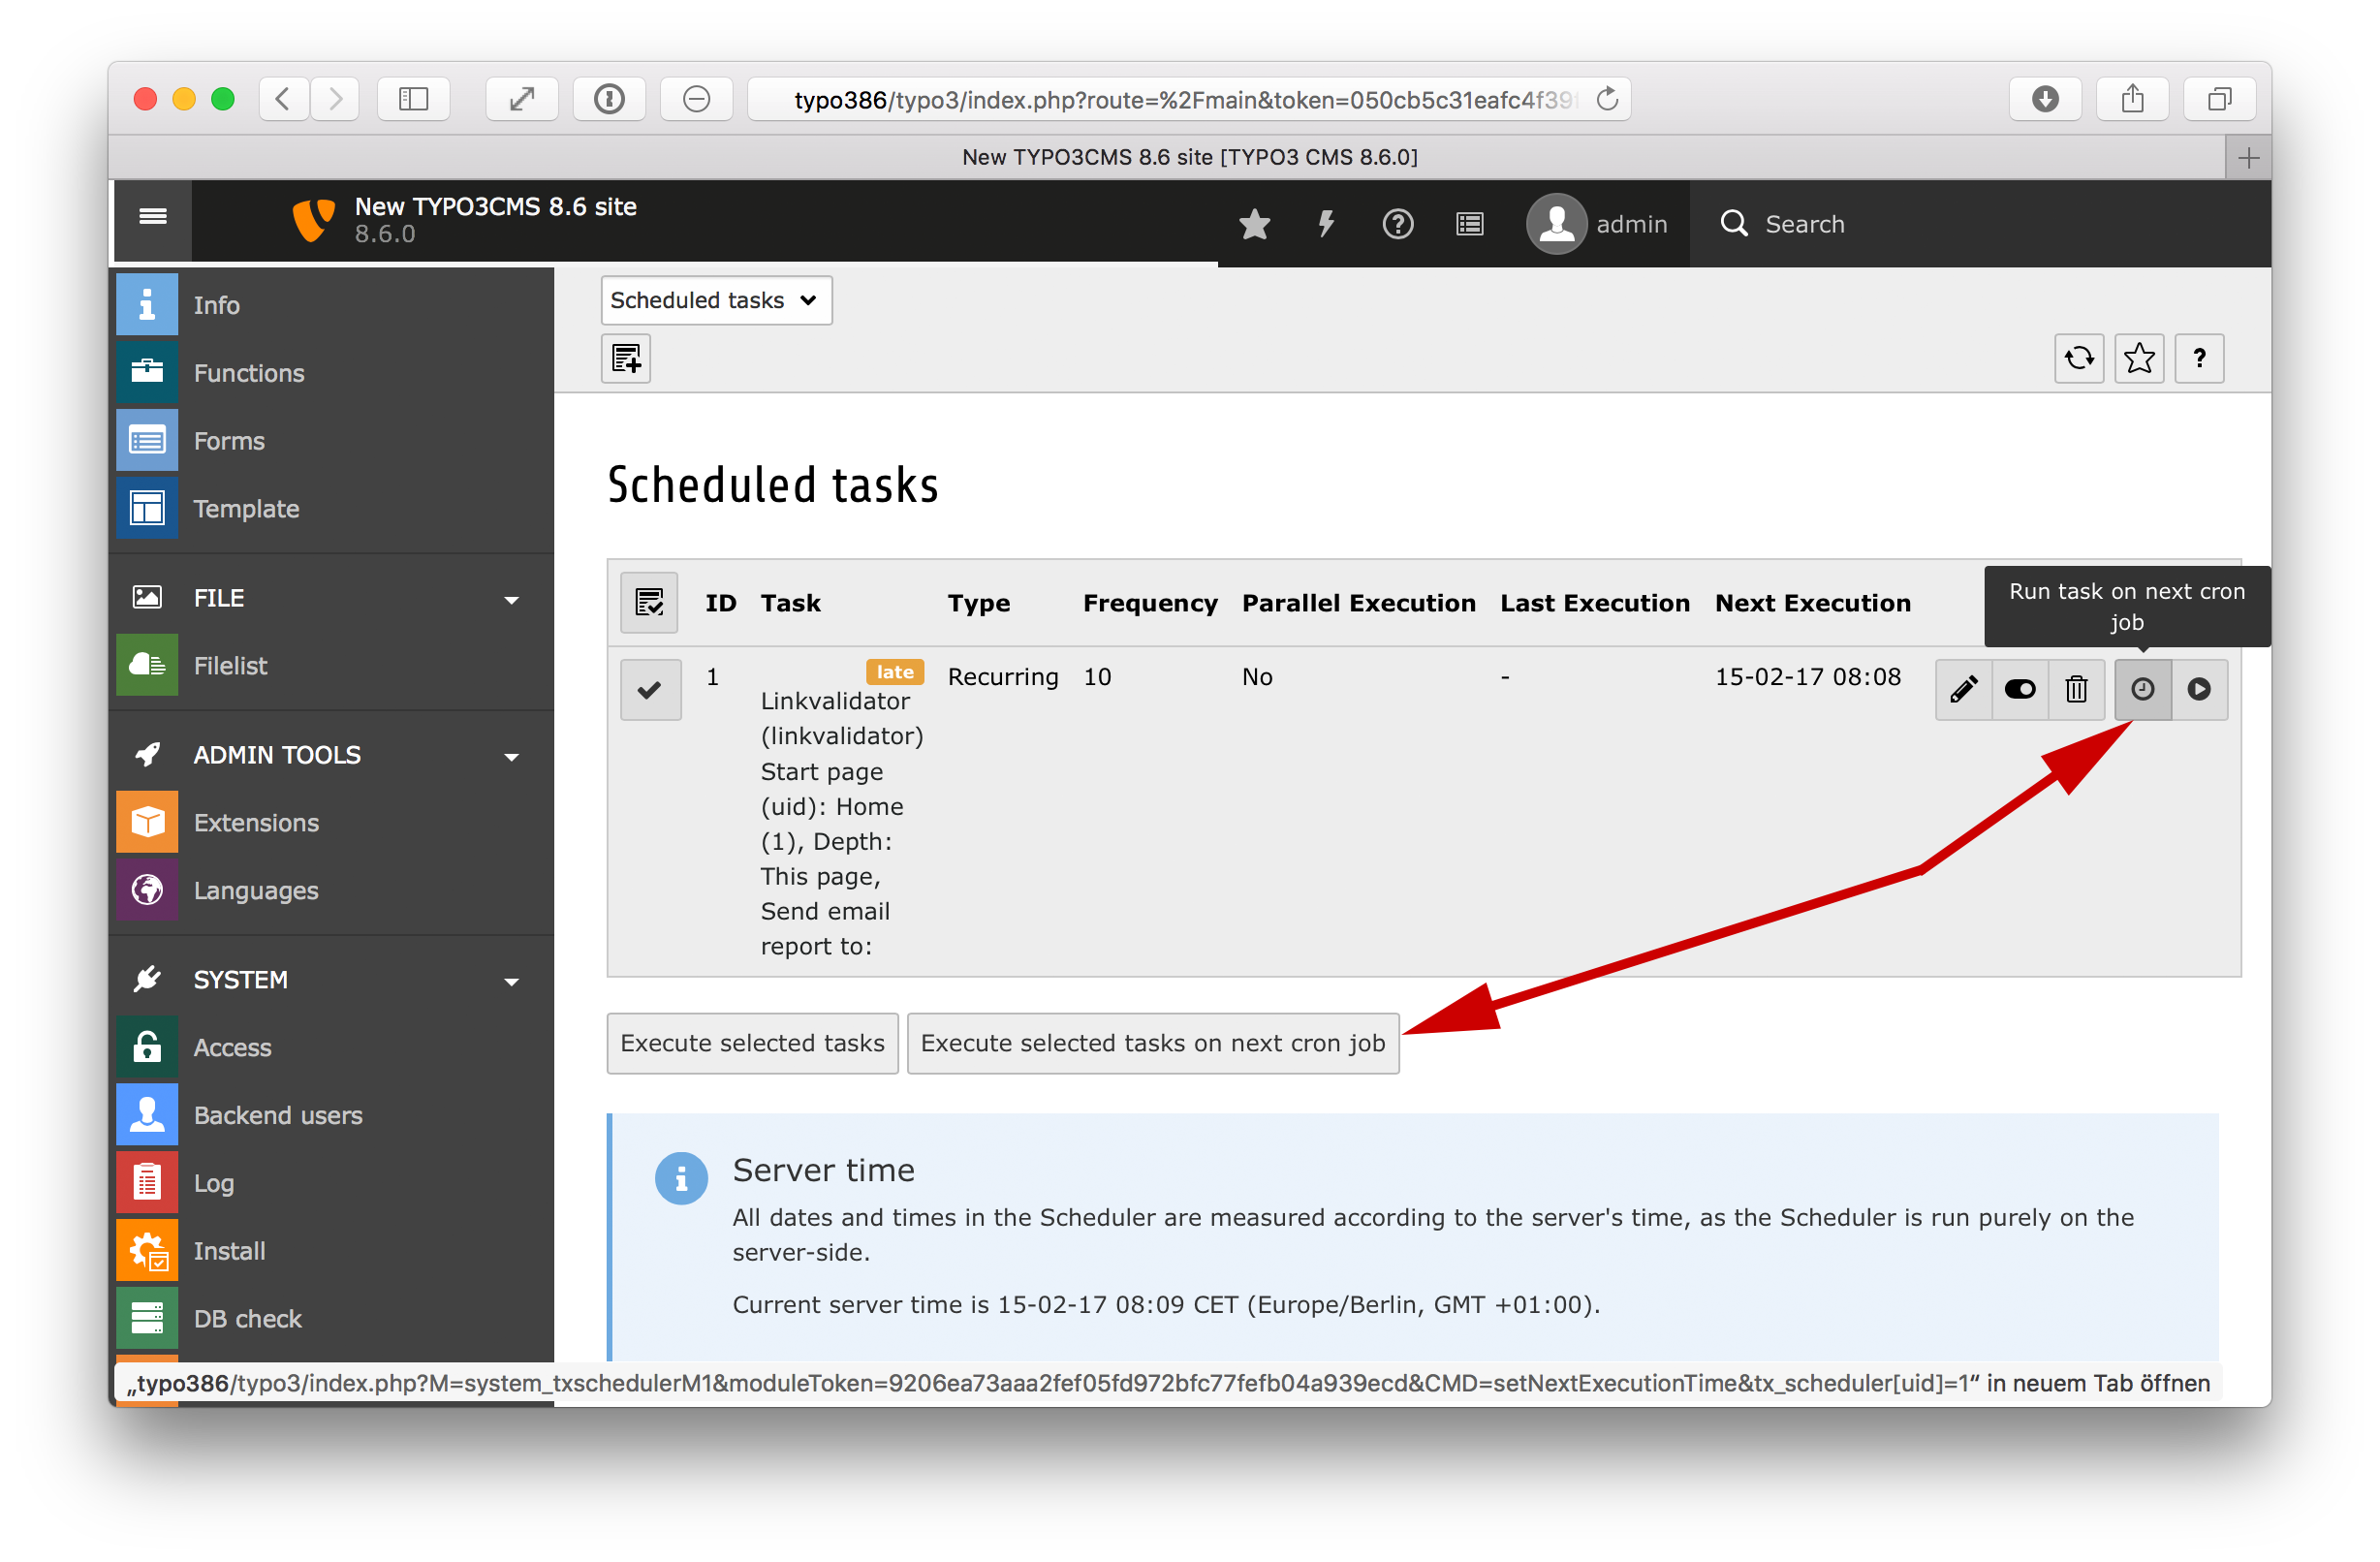
\includegraphics[width=0.99\linewidth]{BackendUserInterface/45537.png}
			\end{figure}
		\end{column}
	\end{columns}

\end{frame}

% ------------------------------------------------------------------------------
% LTXE-SLIDE-START
% LTXE-SLIDE-UID:		233dc011-b09dd1ec-92ddffa1-b1688eff
% LTXE-SLIDE-ORIGIN:	b6d6054e-21291d35-479a0095-a6e82a4f English
% LTXE-SLIDE-TITLE:		#47135: Paste Icon and Modal
% LTXE-SLIDE-REFERENCE:	!Feature: #51291 - Synchronized field values in localized records
% ------------------------------------------------------------------------------
\begin{frame}[fragile]
	\frametitle{Interfaz de Usuario de Backend}
	\framesubtitle{Pegar Iconos y Modal}

	Tan pronto como el portapapeles normal contiene un ítem, un icono único de pegar aparece disponible
	en el módulo de página. Cuando el usuario clica sobre el icono, un modal salta para que el usuario
	confirme la acción.

	\begin{figure}\vspace{-0.2cm}
		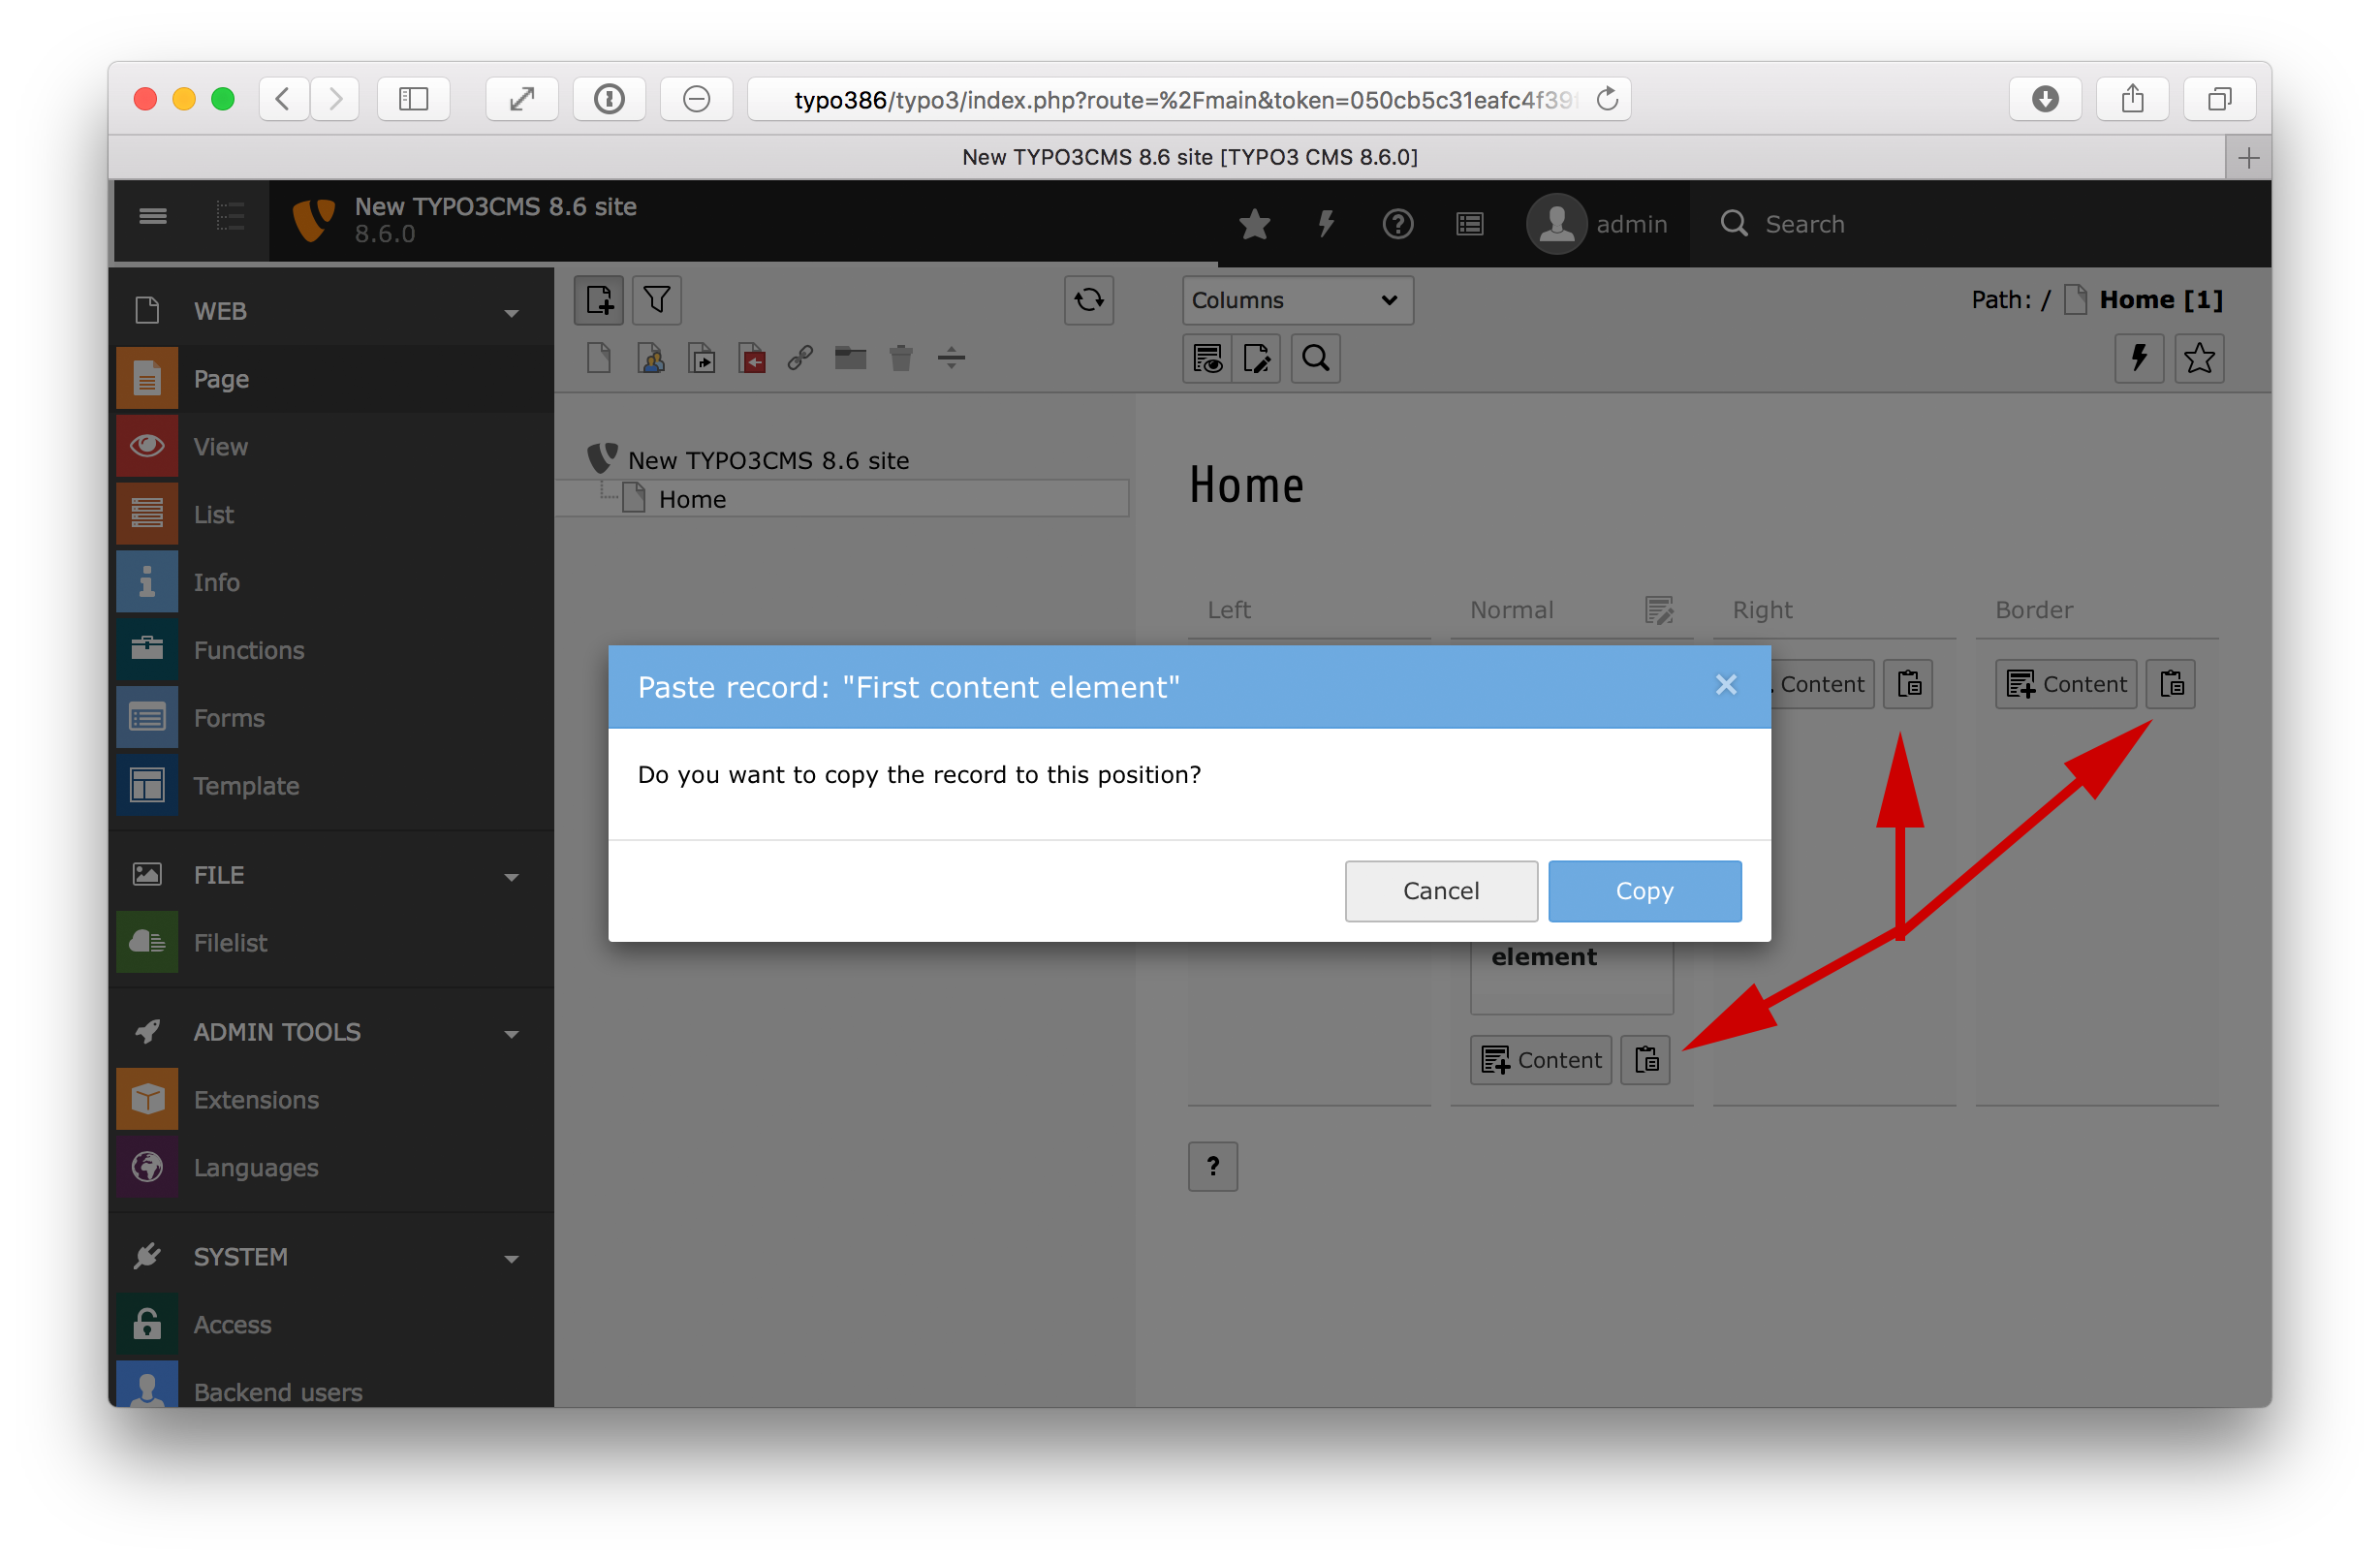
\includegraphics[width=0.63\linewidth]{BackendUserInterface/47135.png}
	\end{figure}

\end{frame}

% ------------------------------------------------------------------------------
% LTXE-SLIDE-START
% LTXE-SLIDE-UID:		f1360f5f-f58bbb1d-766932d0-997cfd6a
% LTXE-SLIDE-ORIGIN:	b31e455f-fce042ed-e3670436-9e72983c English
% LTXE-SLIDE-TITLE:		#67243: Folding of Scheduler Task Groups
% LTXE-SLIDE-REFERENCE:	!Feature: #67243 - Implement folding of scheduler task groups
% ------------------------------------------------------------------------------
\begin{frame}[fragile]
	\frametitle{Interfaz de Usuario de Backend}
	\framesubtitle{Plegado de Grupos de Tareas del Programador}

	Cuando los grupos de tareas se usan, las tareas se despliegan agrupadas en la lista de tareas.
	Cliqueando en la fila con el título del grupo esconde o muestra las tareas del grupo ahora.

	\begin{figure}\vspace{-0.3cm}
		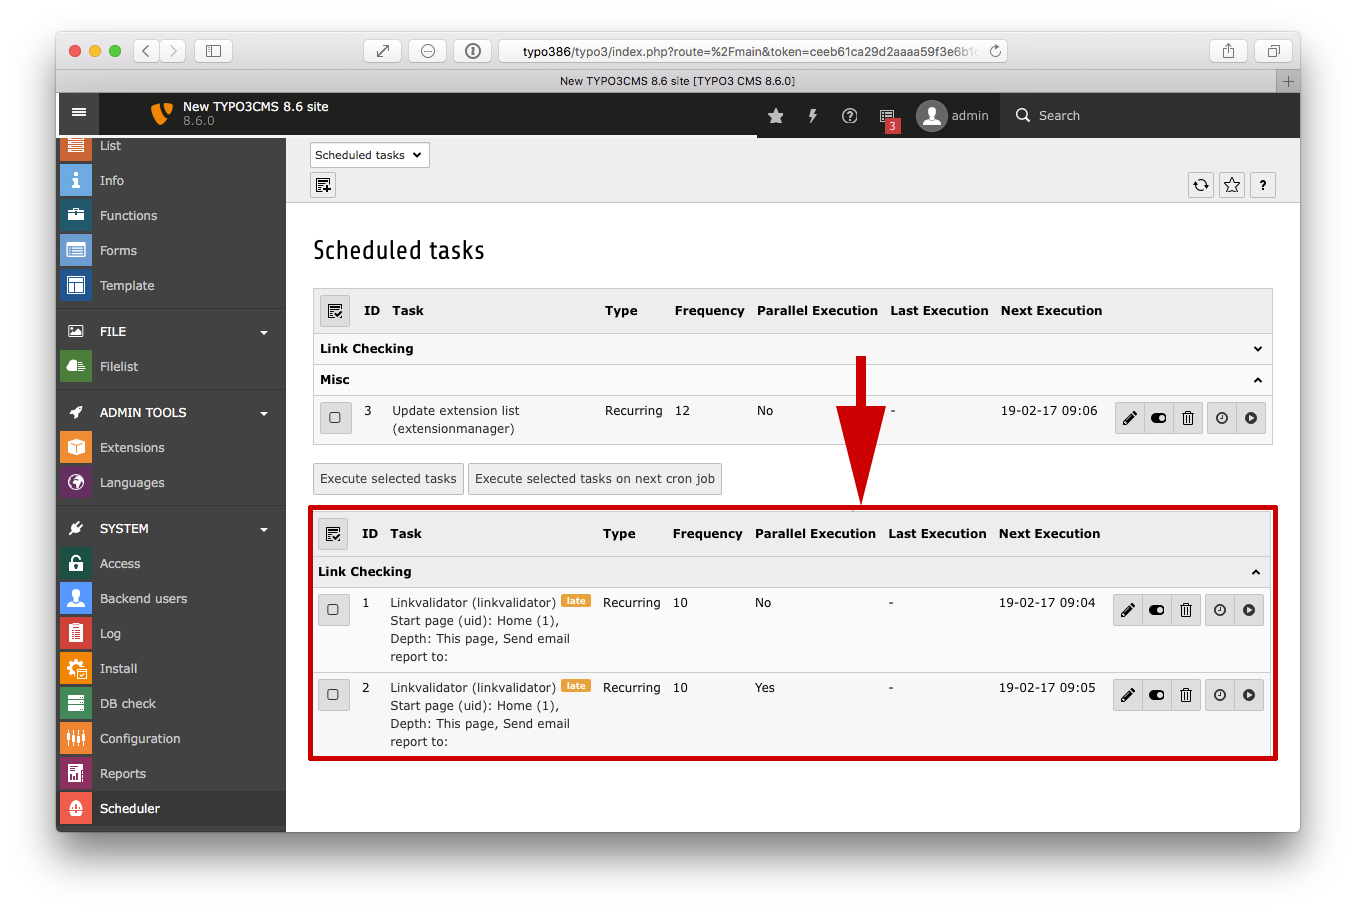
\includegraphics[width=0.60\linewidth]{BackendUserInterface/67243.png}
	\end{figure}

\end{frame}

% ------------------------------------------------------------------------------
% LTXE-SLIDE-START
% LTXE-SLIDE-UID:		d247e044-bac579ea-6da1d968-7db1abf1
% LTXE-SLIDE-ORIGIN:	14fe5a0b-2a22a6ce-325b5de1-ef26ce50 English
% LTXE-SLIDE-TITLE:		#69572: Page Module Notice
% LTXE-SLIDE-REFERENCE:	!Feature: #69572 - Page module Notice "Content is also shown on:"
% ------------------------------------------------------------------------------
\begin{frame}[fragile]
	\frametitle{Interfaz de Usuario de Backend}
	\framesubtitle{Aviso de Módulo de Página "Se muestra también contenido en"}

	\begin{columns}[T]
		\begin{column}{.3\textwidth}
			Cuando el contenido de página se hereda de una página diferente vía "Mostrar contenido de página",
			se despliega un aviso en la página que está extrayendo contenido a una página diferente.
		\end{column}

		\begin{column}{.7\textwidth}
			\begin{figure}\vspace*{-0.6cm}
				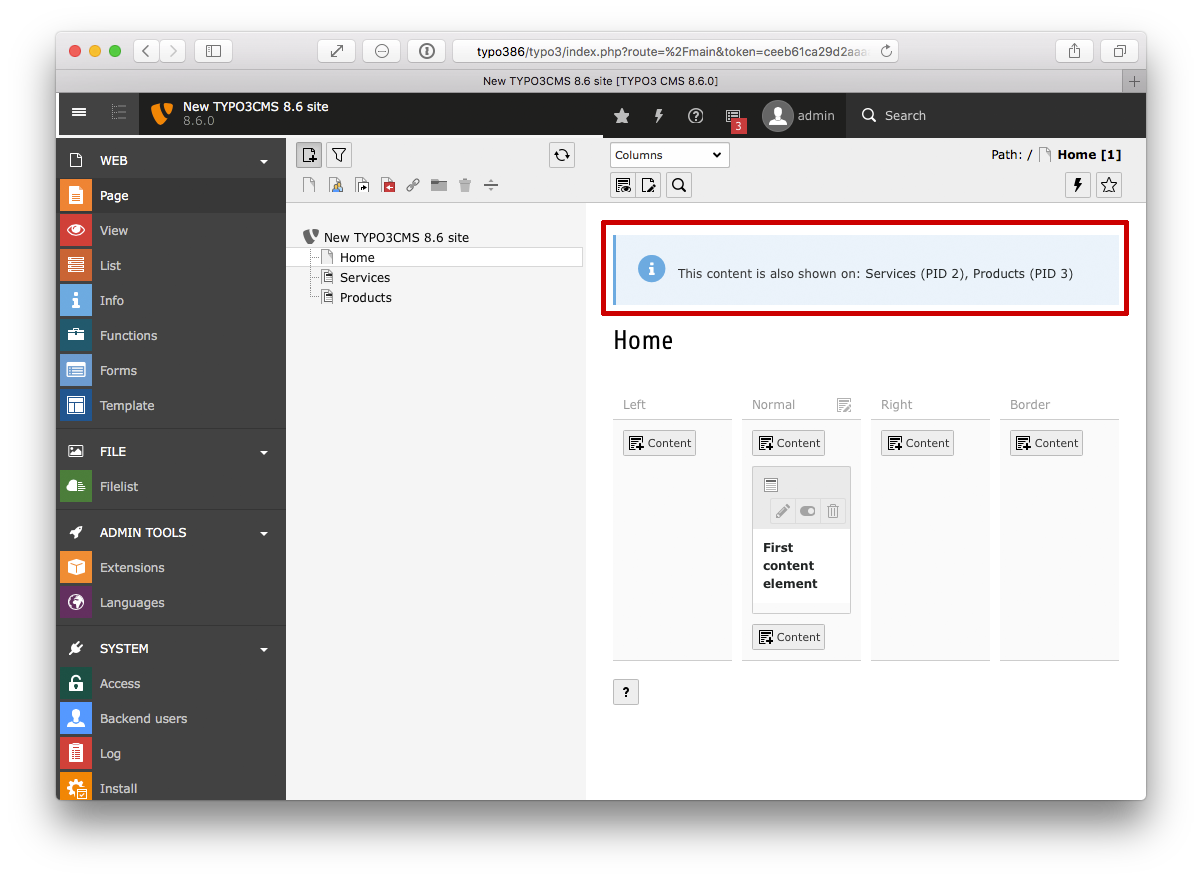
\includegraphics[width=\linewidth]{BackendUserInterface/69572.png}
			\end{figure}
		\end{column}
	\end{columns}

\end{frame}

% ------------------------------------------------------------------------------
% LTXE-SLIDE-START
% LTXE-SLIDE-UID:		e89d3fe3-4b9cd573-c0ec3b0e-9728b7f6
% LTXE-SLIDE-ORIGIN:	23a4baef-462e7d0c-c8cd4cfc-9dac1f99 English
% LTXE-SLIDE-TITLE:		#75880: Image Manipulation - Multiple Cropping Variants
% LTXE-SLIDE-REFERENCE:	!Feature: #75880 - Implement multiple cropping variants in image manipulation tool
% ------------------------------------------------------------------------------
\begin{frame}[fragile]
	\frametitle{Interfaz de Usuario de Backend}
	\framesubtitle{Manipulación de Imagen - Variantes de Recorte Múltiple}

	La Herramienta de Manipulación de Imagen es ahora capaz de manejar múltiples variantes de recorte (si se configuran).
	Los usuarios pueden también seleccionar un área de enfoque, que está siempre dentro del área de recorte y marca el área
	de la imagen que debe ser visible % -- beware of text flow here, it continues in the column

	\begin{columns}[T]
		\begin{column}{.35\textwidth}
			para que la imagen transporte su significado.
			Para dar a los editores una pista de qué área de la imagen es usada por otros DOM-Elements como cabeceras,
			al seleccionar un área de recorte, es posible definir las denominadas múltiples área de envoltura.
		\end{column}

		\begin{column}{.65\textwidth}
			\begin{figure}\vspace*{-0.6cm}
				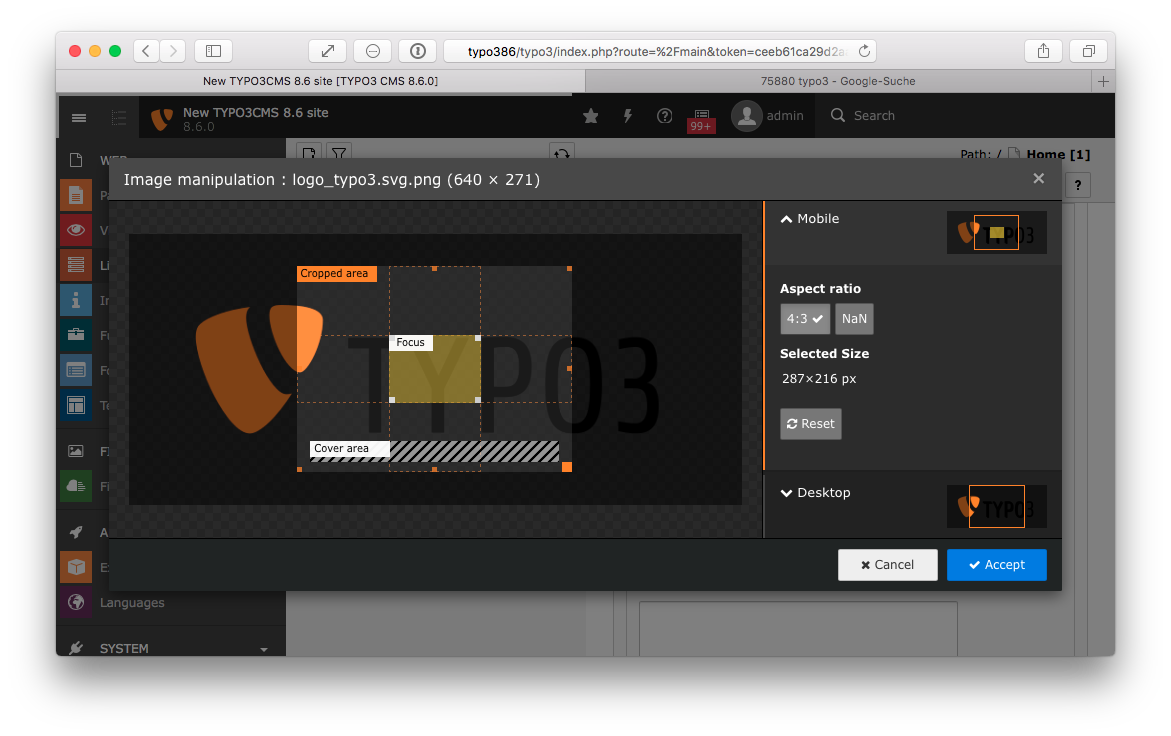
\includegraphics[width=0.99\linewidth]{BackendUserInterface/75880.png}
			\end{figure}
		\end{column}
	\end{columns}

\end{frame}

% ------------------------------------------------------------------------------
% LTXE-SLIDE-START
% LTXE-SLIDE-UID:		d5103022-015f7ded-19db5988-f37663ad
% LTXE-SLIDE-ORIGIN:	8f2f695d-f5c6a8bf-5700cf34-d6389ce8 English
% LTXE-SLIDE-TITLE:		#79235: Delete Similar Errors (sys_log)
% LTXE-SLIDE-REFERENCE:	!Feature: #79235 - Add button to delete similar errors from sys_log
% ------------------------------------------------------------------------------
\begin{frame}[fragile]
	\frametitle{Interfaz de Usuario de Backend}
	\framesubtitle{Borrar Errores Similares de \texttt{sys\_log}}

	El módulo de log de TYPO3 ahora muestra un botón para borrar errores múltiples a la vez basados en el
	campo \texttt{details} de la tabla \texttt{sys\_log}. Esto resulta útil cuando arreglaste
	un error que spameaba el log antes.

	\begin{figure}\vspace{-0.2cm}
		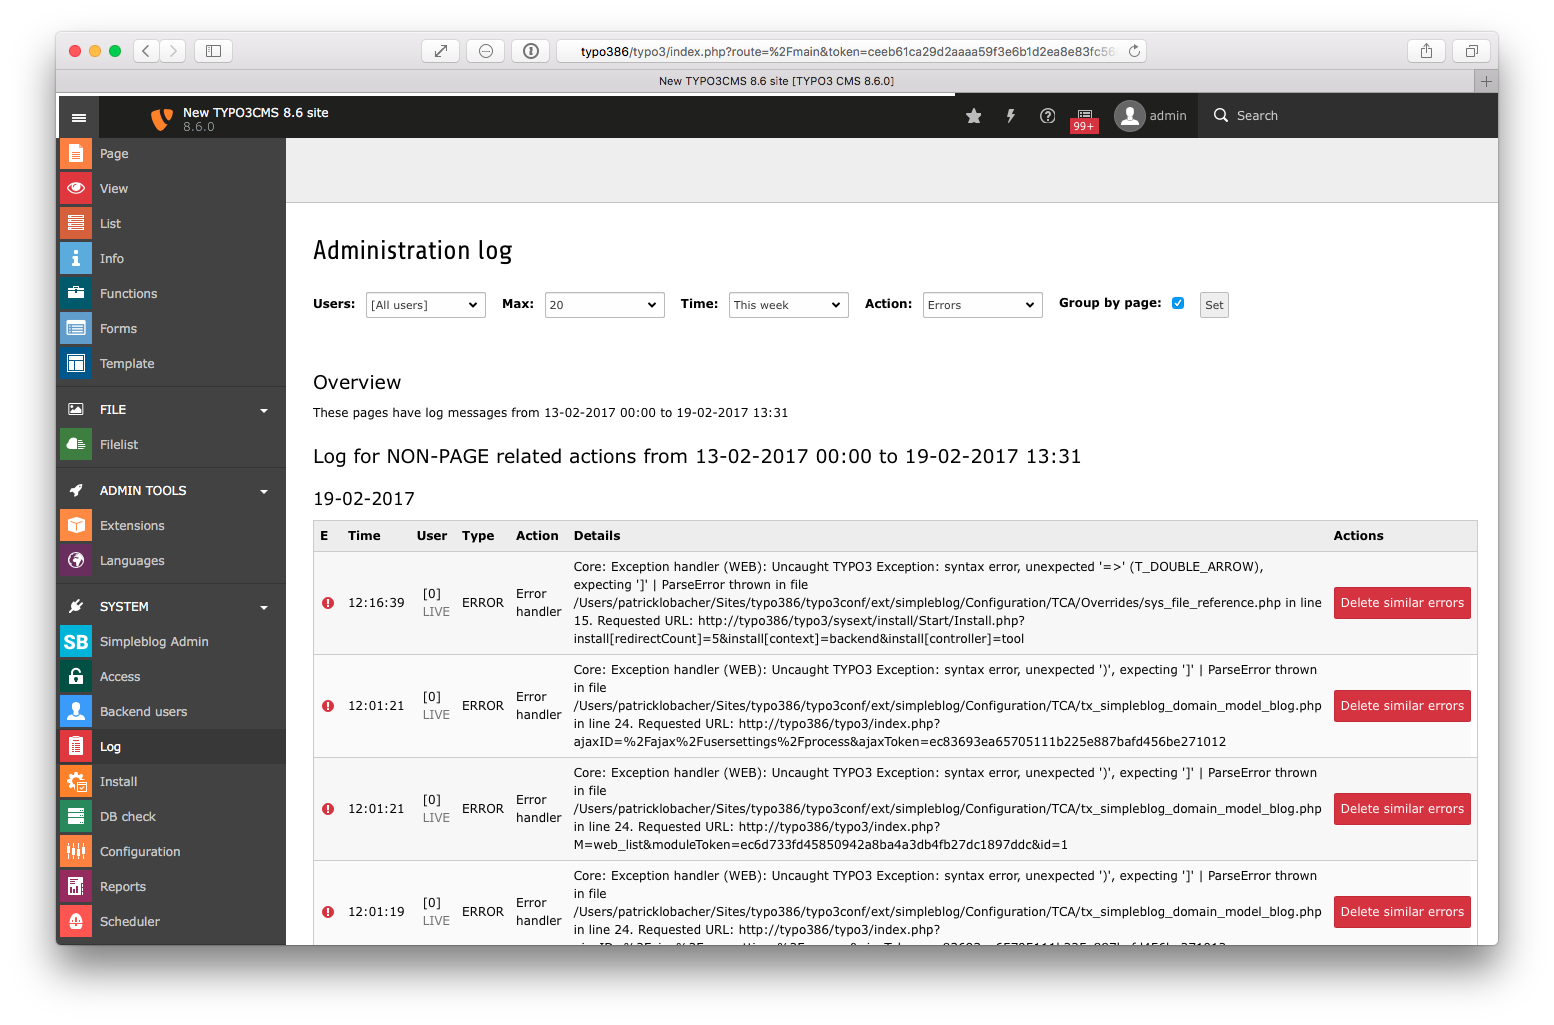
\includegraphics[width=0.60\linewidth]{BackendUserInterface/79235.png}
	\end{figure}

\end{frame}

% ------------------------------------------------------------------------------
% LTXE-SLIDE-START
% LTXE-SLIDE-UID:		d5fd6f12-a19b769e-49299438-0ba76327
% LTXE-SLIDE-ORIGIN:	fc878ad9-7b163d51-e579b8b3-9cbe41d9 English
% LTXE-SLIDE-TITLE:		#79467: Form settings button
% LTXE-SLIDE-REFERENCE:	!Feature: #79467 - EXT:form - add form settings button to module header
% ------------------------------------------------------------------------------
\begin{frame}[fragile]
	\frametitle{Interfaz de Usuario de Backend}
	\framesubtitle{\texttt{EXT:form}: añadir botón de ajustes del formulario a la cabecera del módulo}

	Un nuevo botón ha sido añadido a la cabecera del módulo del editor de formulario.
	Cliqueando sobre este botón muestra los ajustes de formulario dentro del inspector.

	\begin{figure}\vspace{-0.2cm}
		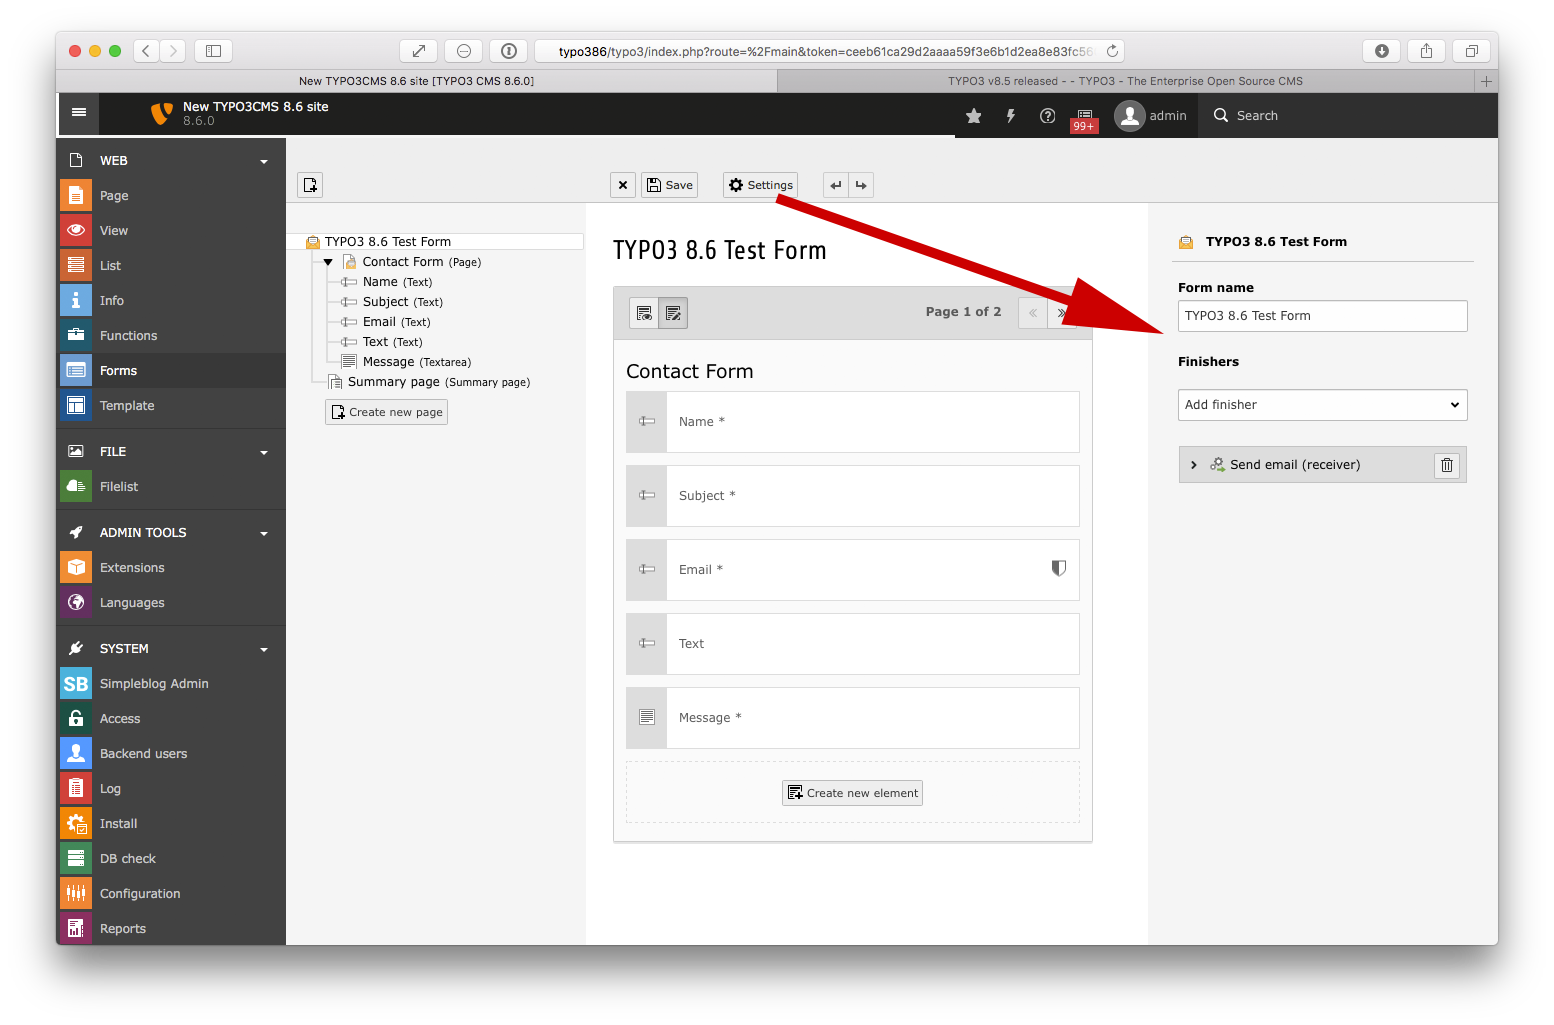
\includegraphics[width=0.675\linewidth]{BackendUserInterface/79467.png}
	\end{figure}

\end{frame}

% ------------------------------------------------------------------------------
% LTXE-SLIDE-START
% LTXE-SLIDE-UID:		8a66332d-30550d04-7eee8395-51f7c60e
% LTXE-SLIDE-ORIGIN:	e1759d2e-8cc138ca-40ce6a34-65354b0e English
% LTXE-SLIDE-TITLE:		#79531: EXT:form - Add multiselect inspector editor
% LTXE-SLIDE-REFERENCE:	!Feature: #79531 - EXT:form - Add multiselect inspector editor
% ------------------------------------------------------------------------------
\begin{frame}[fragile]
	\frametitle{Interfaz de Usuario de Backend}
	\framesubtitle{{EXT:form}: Añadir editor de inspector de multiselección}

	\begin{columns}[T]
		\begin{column}{0.35\textwidth}
			Un nuevo editor de inspección, es decir un nuevo tipo de campo del editor de formulario, ha sido añadido.
			Si se aplica, campos de multiselección pueden ser añadidos al inspector.
			Un campo de multiselección permite la selección de múltiples propiedades meta para un campo
			y las almacena en la ruta de la propiedad definida.
		\end{column}

		\begin{column}{0.65\textwidth}
			\begin{figure}\vspace*{-0.6cm}
				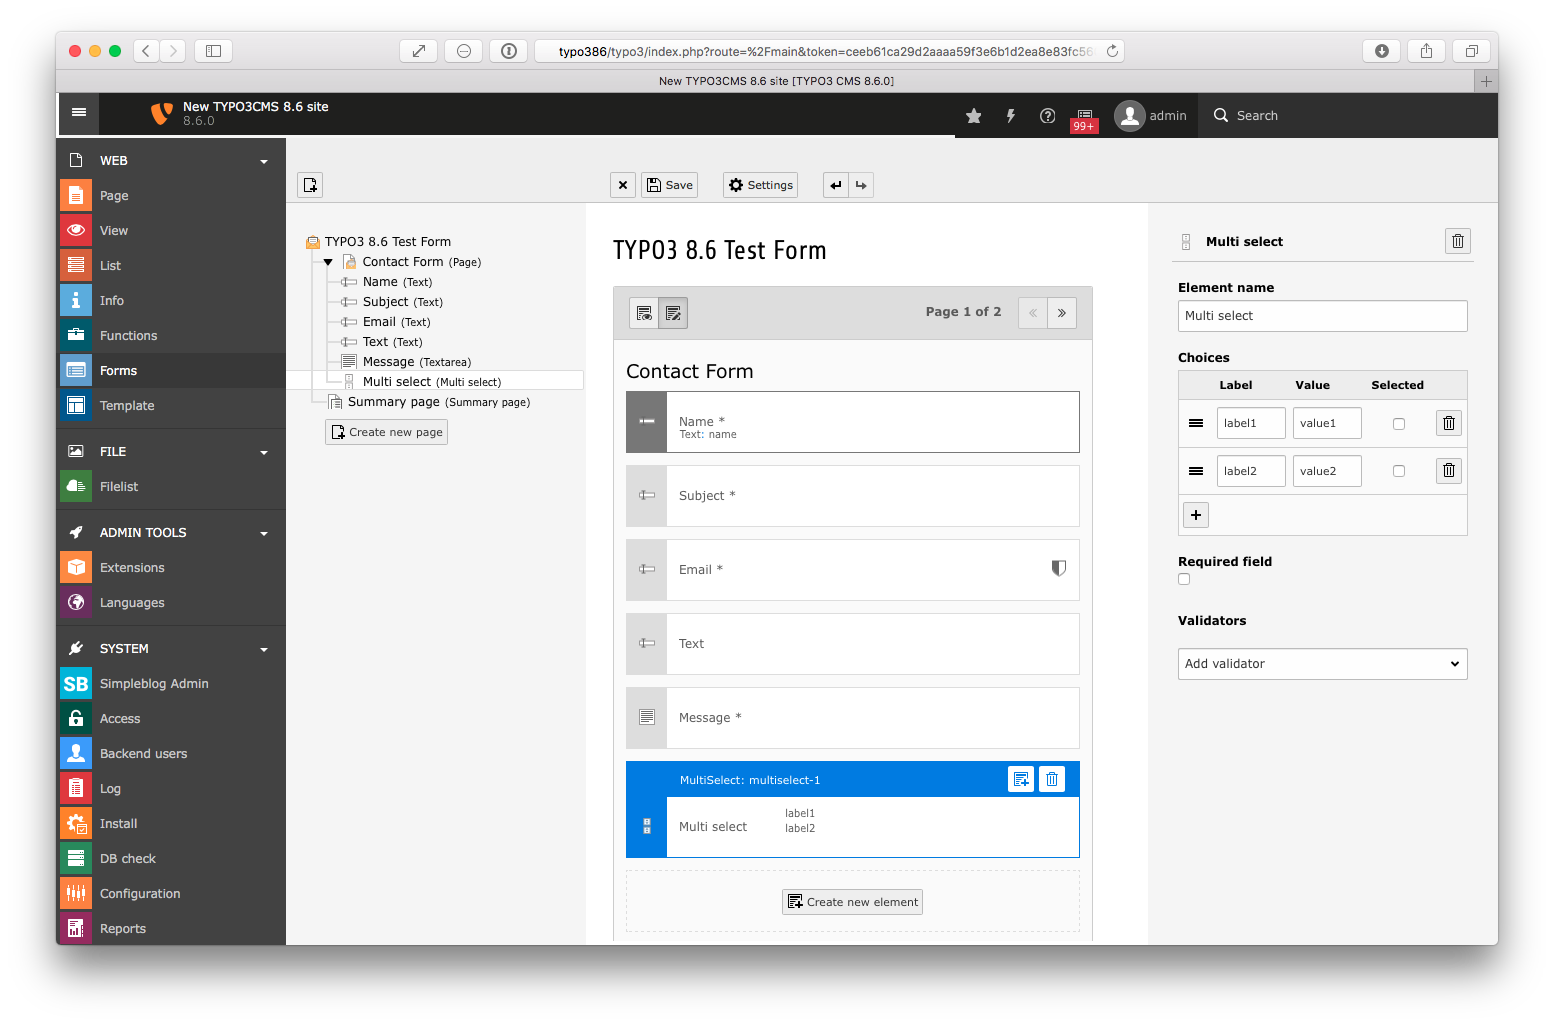
\includegraphics[width=0.99\linewidth]{BackendUserInterface/79531.png}
			\end{figure}
		\end{column}
	\end{columns}

\end{frame}

% ------------------------------------------------------------------------------
% LTXE-SLIDE-START
% LTXE-SLIDE-UID:		76d16d16-4104897d-16c6647a-1337da4e
% LTXE-SLIDE-ORIGIN:	f6756002-b9aac45f-9460b472-1da819b5 English
% LTXE-SLIDE-TITLE:		#79521: Show list of failed input elements in FormEngine
% LTXE-SLIDE-REFERENCE:	!Feature: #79521 - Show list of failed input elements in FormEngine
% ------------------------------------------------------------------------------
\begin{frame}[fragile]
	\frametitle{Interfaz de Usuario de Backend}
	\framesubtitle{Mostrar lista de elementos de entrada de fallo en FormEngine}

	\begin{columns}[T]
		\begin{column}{.35\textwidth}
			Cuando la validación de campos de entrada del FormEngine falla, un botón es ahora desplegado en
			la barra de bottones en la cabecera del módulo de documento. Al clicar el botón se despliega una lista de
			todos los elementos de entrada cuya validación falló. Clicar en un campo de dicha lista
			automáticamente pone el enfoque del campo en el formulario.
		\end{column}

		\begin{column}{.65\textwidth}
			\begin{figure}\vspace*{-0.6cm}
				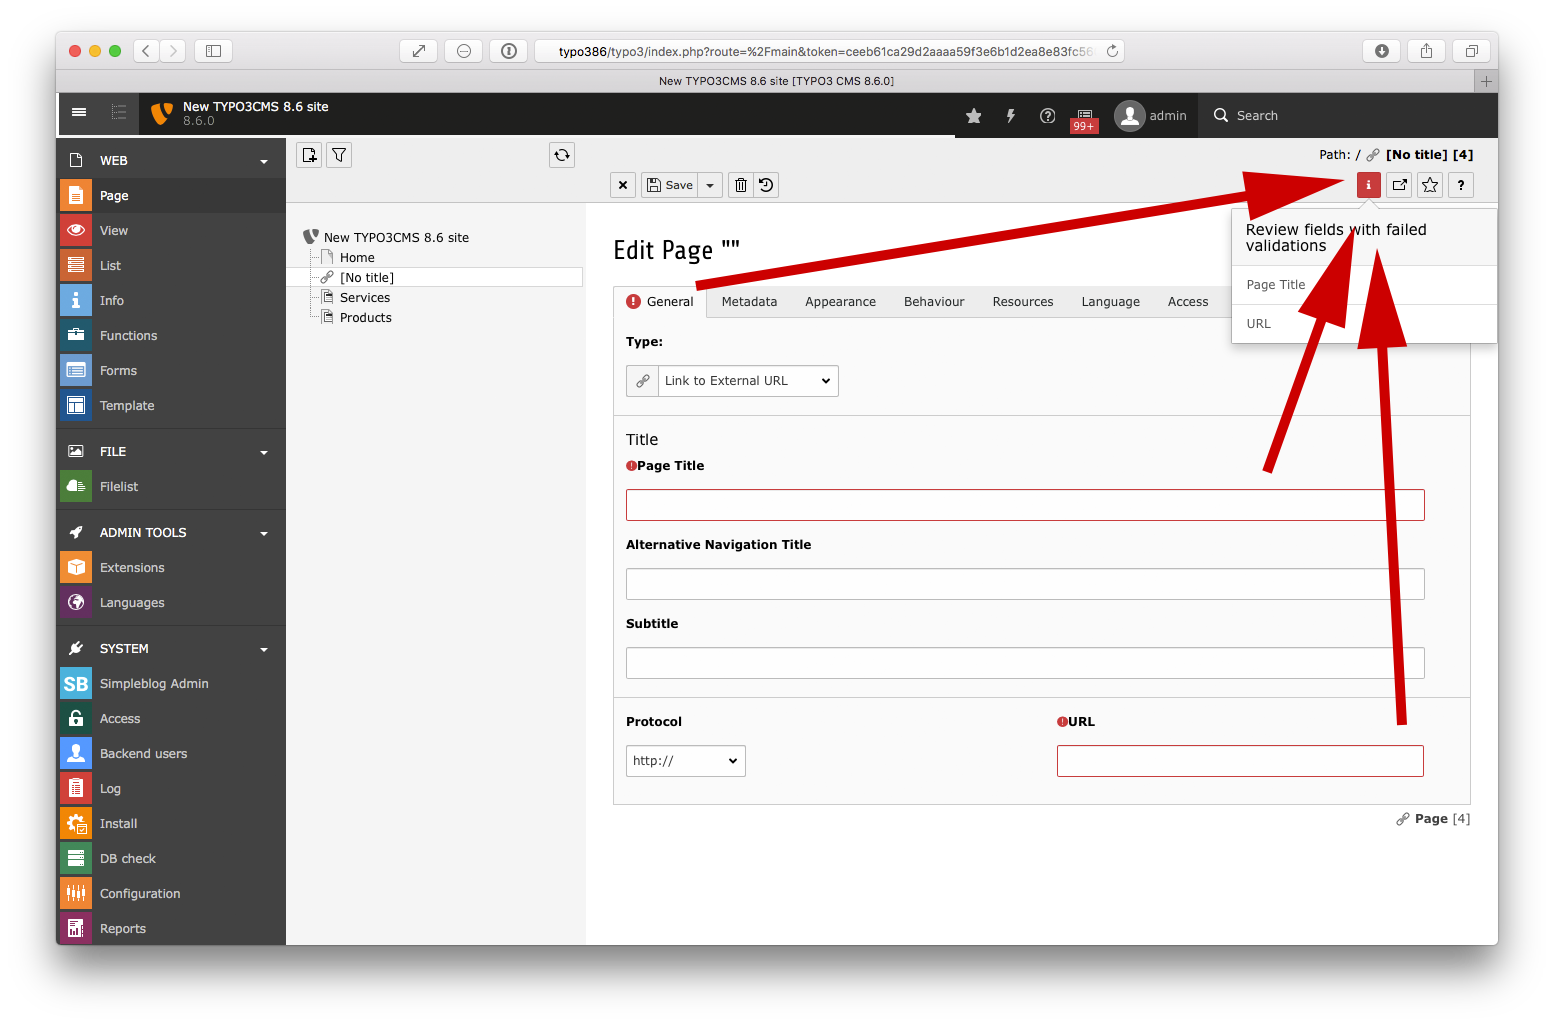
\includegraphics[width=0.99\linewidth]{BackendUserInterface/79521.png}
			\end{figure}
		\end{column}
	\end{columns}

\end{frame}

% ------------------------------------------------------------------------------
% LTXE-SLIDE-START
% LTXE-SLIDE-UID:		c32b226f-a862e875-a80d86ba-6a09ac13
% LTXE-SLIDE-ORIGIN:	749a055b-02003192-92f2631e-39abcc95 English
% LTXE-SLIDE-TITLE:		#79622: Dedicated content elements for menus
% LTXE-SLIDE-REFERENCE:	!Breaking: #79622 - Dedicated content elements for menus
% ------------------------------------------------------------------------------
\begin{frame}[fragile]
	\frametitle{Interfaz de Usuario de Backend}
	\framesubtitle{Elementos de contenido dedicados para menús}

	Para mejor mantenimiento el elemento de contenido de menú existente ha sido
	dividido en elementos de contenido dedicados.

	\begin{figure}\vspace{-0.2cm}
		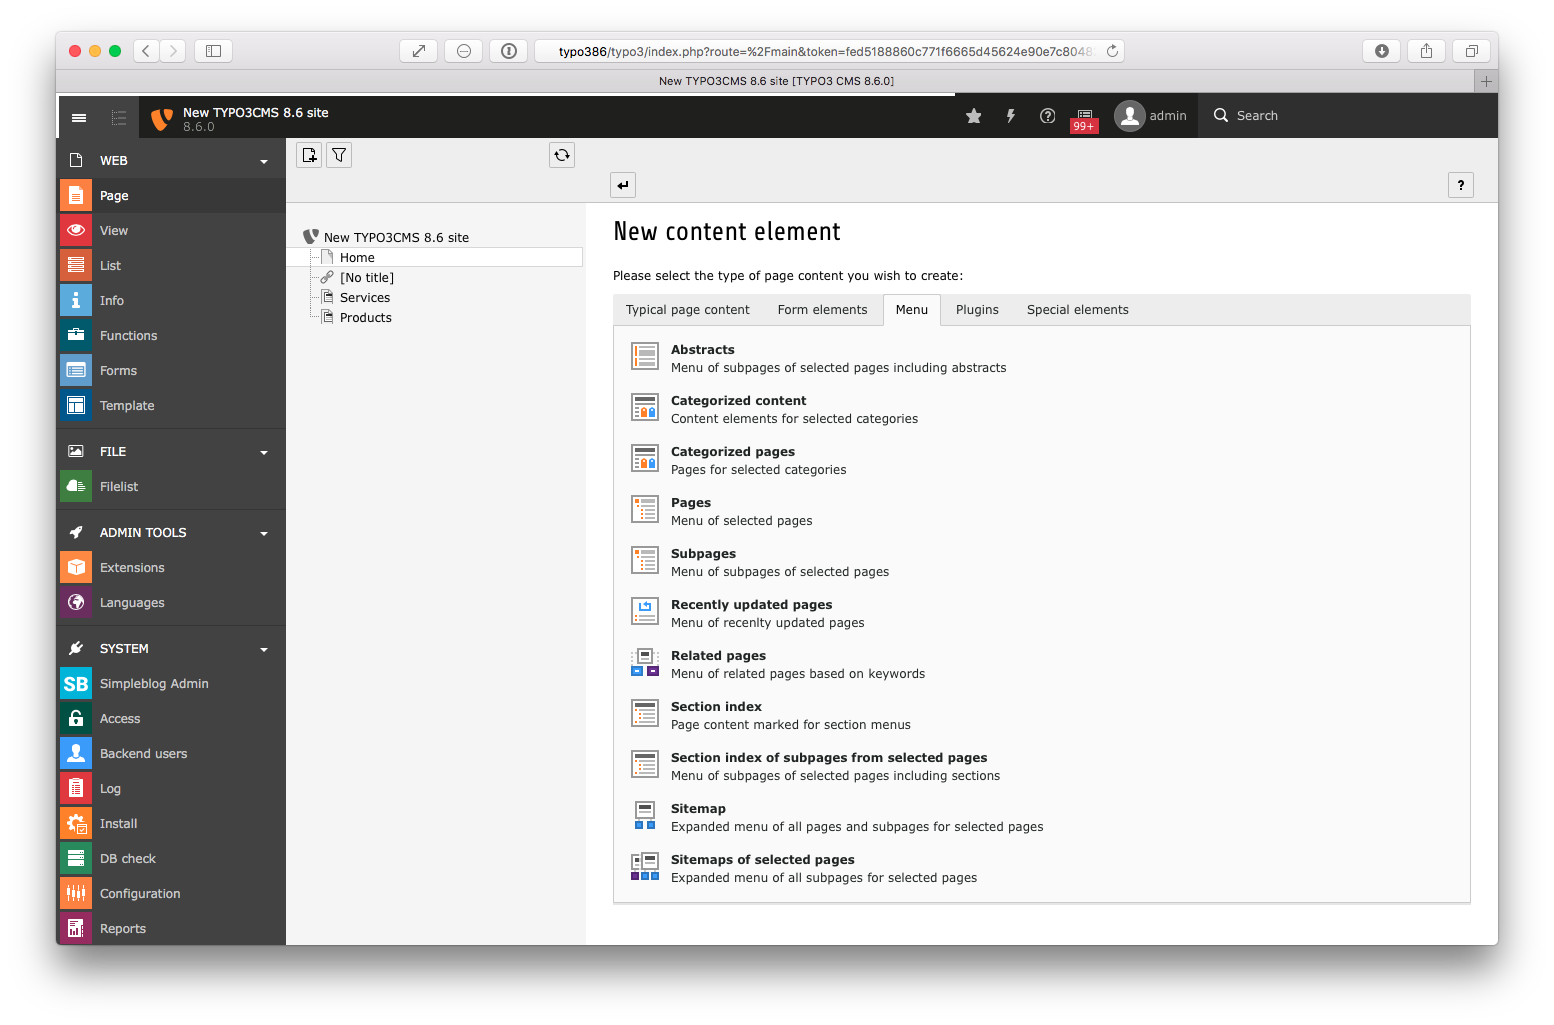
\includegraphics[width=0.68\linewidth]{BackendUserInterface/79622.png}
	\end{figure}

\end{frame}

% ------------------------------------------------------------------------------
